\def\layersep{2.5cm}

\begin{figure}[H]
\center
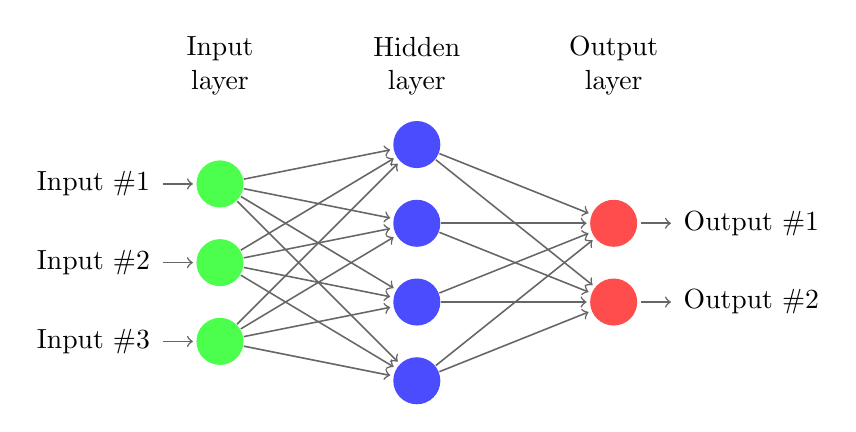
\begin{tikzpicture}[shorten >=1pt,->,line width=0.2mm,draw=black!60, node distance=\layersep]
    \tikzstyle{every pin edge}=[<-,shorten <=1pt]
    \tikzstyle{neuron}=[circle,fill=black!25,minimum size=17pt,inner sep=0pt]
    \tikzstyle{input neuron}=[neuron, fill=green!70];
    \tikzstyle{output neuron}=[neuron, fill=red!70];
    \tikzstyle{hidden neuron}=[neuron, fill=blue!70];
    \tikzstyle{annot} = [text width=4em, text centered]

    % Draw the input layer nodes
    %\foreach \name / \y in {1,...,4}
    % This is the same as writing \foreach \name / \y in {1/1,2/2,3/3,4/4}
    \node[input neuron, pin=left:Input \#1] (I-1) at (0,-1.5) {};
    \node[input neuron, pin=left:Input \#2] (I-2) at (0,-2.5) {};
    \node[input neuron, pin=left:Input \#3] (I-3) at (0,-3.5) {};

    % Draw the hidden layer 1 nodes
    \node[hidden neuron] (H-1) at (\layersep,-1) {};
    \node[hidden neuron] (H-2) at (\layersep,-2) {};
    \node[hidden neuron] (H-3) at (\layersep,-3) {};
    \node[hidden neuron] (H-4) at (\layersep,-4) {};

    % Draw the output layer node
    \node[output neuron,pin={[pin edge={->}]right:Output \#1}] (O-1) at (2*\layersep,-2) {};
    \node[output neuron,pin={[pin edge={->}]right:Output \#2}] (O-2) at (2*\layersep,-3) {};

    % Connect every node in the input layer with every node in the
    % hidden layer.
    \path (I-1) edge (H-1);
    \path (I-2) edge (H-1);
    \path (I-3) edge (H-1);
    \path (I-1) edge (H-2);
    \path (I-2) edge (H-2);
    \path (I-3) edge (H-2);
    \path (I-1) edge (H-3);
    \path (I-2) edge (H-3);
    \path (I-3) edge (H-3);
    \path (I-1) edge (H-4);
    \path (I-2) edge (H-4);
    \path (I-3) edge (H-4);
    
    % Connect every node in the hidden layer with the output layer
    \path (H-1) edge (O-1);
    \path (H-1) edge (O-2);
    \path (H-2) edge (O-1);
    \path (H-2) edge (O-2);
    \path (H-3) edge (O-1);
    \path (H-3) edge (O-2);
    \path (H-4) edge (O-1);
    \path (H-4) edge (O-2);

    % Annotate the layers
    \node[annot,above of=H-1, node distance=1cm] (hl) {Hidden layer};
    \node[annot,left of=hl] {Input layer};
    \node[annot,right of=hl] {Output layer};
\end{tikzpicture}
\caption{Multilayer Perceptron with three inputs and two outputs. \label{fig:mlp}}
\end{figure}